\documentclass[a4paper]{report} % estilo do documento

\usepackage[utf8]{inputenc} %encoding do ficheiro
\usepackage[portuges]{babel} % para língua portuguesa
\usepackage{graphicx} % para importar imagens


\begin{document}

\begin{figure} [t]
    \centering
    
\includegraphics [scale = 0.1]{um.png}
\end{figure}
    
\title {\huge Relatório do "Micro Machines"}
\author{Grupo 13\\
João Sampaio e José Ferreira}

\date{31 de Dezembro de 2017}

\maketitle

\tableofcontents

\listoffigures

\listoftables

%% Introdução
\chapter{Introdução}
\section{Contextualização}

    Tem data de 1991, o lançamento da primeira versão do lendário jogo de 
    miniaturas de carros, o intitulado "Micro Machines".
    
    Capaz de relembrar a criança que gosta de brincar com pequenas miniaturas, a sua inovação na época de lançamento, fez com que este fosse uns dos primeiros grandes sucessos no mundo do videojogos.
    
    No 1º semestre do curso de MIEI, do ano letivo 2017/2018, em "Laboratórios de Informática I" foi pedido ao aluno que faça uma réplica do jogo em questão
    O resultado final será o único elemento de avaliação do aluno na disciplina. 
    
    

 \ldots
  
  \section{Motivação}
    
    Na primeira aula da Unidade Curricular, dizer a um aluno que neste semestre não seria avaliado através de um teste foi um belo trunfo para despertar o seu interesse. Do cômputo geral, o estudante de qualquer Engenharia gosta mais do trabalho prático, pelo que não foi dificil fazer com que exitisse bastante empenho e dedicação para a apresentação de um bom resultado.
    Para além disso, o trabalho solicitado permite o desenvolvimento das capacidades de qualquer informático.

 \newpage
  
 
 \ldots
 \section{Objectivos}
    
    Trabalhando em pares, a estes compete o cumprimento dos objetivos propostos pelos docentes, em 6 tarefas distintas.
    O projeto divide-se em 2 fases. 
    
    Na 1ºfase, pretende-se construir mapas e validá-los segundo um conjunto e critérios fornecidos, Tarefa 1 e 2 ,respectivamente. Dentro dela ainda se inclui a Tarefa 3, onde é implementada a movimentação do carro. 
    
    Na 2ºfase, e ainda envolvendo a mecânica do jogo, com a Tarefa 4 obtem-se a atualização do estado do carro. Com a ajuda do Gloss, na Tarefa 5 entra a computação gráfica no executável do "Micro Machines". Por fim, na Tarefa 6 é programada uma estratégia de jogo para os bots.
    
    Com este documento, espera-se realizar uma explicação sucinta de tudo aquilo que está por detrás do executável do jogo acima referido. Pretende-se expor de forma clara quais foram as linhas orientadoras para a redação do seu código e quais as ferramentas utilizadas para a sua execução.
    
    Mais a mais, será exposto quais as principais dificuldades, bem como quais os métodos encontrados para a sua resolução.
    O objetivo é claro : um leitor muito mais esclarecido sobre a temática abordada.
    
    
   \begin{figure}[h!]
        \centering
        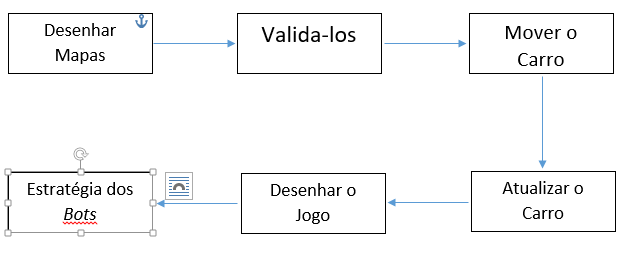
\includegraphics[scale= 0.7]{graficoR.PNG}
        \caption{Esquema dos Objetivos}
        \label{fig:my_label}
    \end{figure}

    \ldots

%% Análise de Requisitos e Especificação do Problema
\chapter{Análise de Requisitos}

\section{Fase 1}
\label{sec:analisefase1}

\subsection{Tarefa 1}

 Os mapas são a base de qualquer jogo de corrida. Dessa forma, faz sentido que a tarefa inicial seja a redação de um código que permita criar qualquer mapa a partir de um caminho dado.
 
 O maior desafio desta Tarefa será fazer com que as diferentes peças (abaixo expostas) se situem no local correto.
 
 \begin{figure} [!htb]
     
     \centering
     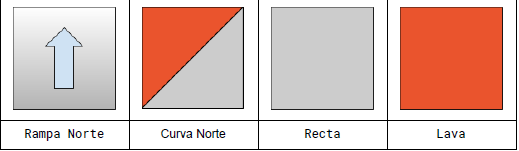
\includegraphics [scale = 0.80] {Lava.PNG}
     \caption{Peças do Mapa}
     \label{fig:my_label}
 
 \end{figure}
 
 Pretende-se definir a função \textbf{constroi}, que através de um \emph{Caminho}, constroi o \emph{Mapa} correspondente.
 
 \begin{verbatim}

constroi :: Caminho -> Mapa

 \end{verbatim}
 \newpage
 
 \subsection{Tarefa 2}
 
 Para assegurar que isso acontece, na Tarefa 2 pretende-se a criação de um algoritmo capaz de averiguar se o mapa é válido.
 
 Todas as hipotéticas situações devem ser tidas em conta. A condição mais relevante, será garantir que o ponto de partida da formação do mapa é também o seu ponto final (condição não assegurada no 3º mapa da figura 2.2).
 
 Pretende-se a elaboração da função \textbf{valida}, que recebe um \emph{Mapa} e devolve um \emph{Bool}.
 
 \begin{verbatim}
    
  valida :: Mapa -> Bool
 
 \end{verbatim}
 
\begin{figure}[h!]
 \begin{center}
 \includegraphics[scale= 0.080] {mapasInvalidos.png}
 \caption{Mapas Inválidos} \label{gdimotes}
 \end{center}
\end{figure}

\begin{figure}[h!]
 \begin{center}
 \includegraphics[scale= 0.080] {mapasV.png}
 \caption{Mapas Válidos} \label{gdimotes}
 \end{center}
\end{figure}
 
\newpage
 
 \subsection{Tarefa 3}
 
 A derradeira etapa desta 1ºfase é a movimentação de um carro. Perante a ação de um jogador, o carro deve mover-se para a posição esperada. É necessário garantir que ocorre sua destruição quando estiver em contacto com a lava. Para além disso, deverá existir ricochete quando a diferença de alturas entre peças é superior a 1.
 
 O objetivo desta Tarefa é definir a função \textbf{movimenta}, que dado um \emph{Tabuleiro}, um \emph{Tempo} e um \emph{Carro},  devolve um \emph{Carro} correspondente. 

\begin{verbatim}
     movimenta :: Tabuleiro -> Tempo -> Carro -> Maybe Carro
     movimenta tab t c = isDestroyed tab (move t c)

\end{verbatim}

\begin{figure}[!h]
    \centering
    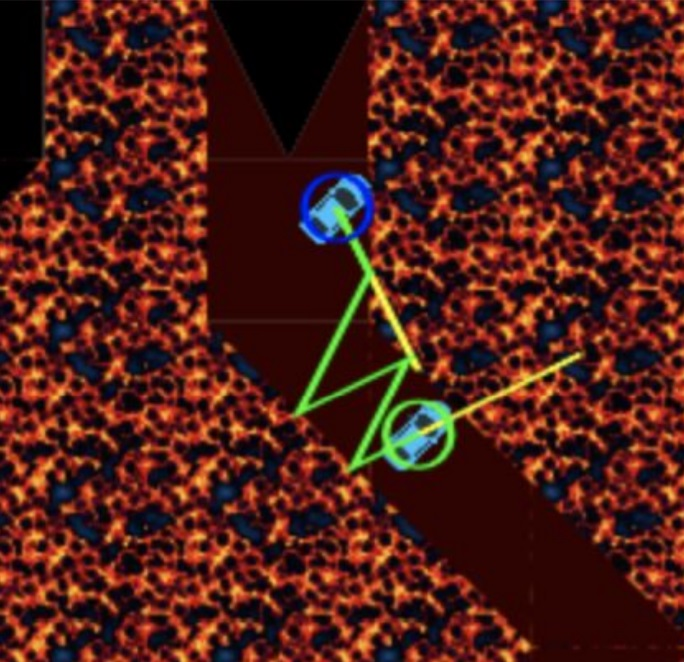
\includegraphics [scale= 0.5]{colisao.jpg}
    \caption{Movimentação do Carro}
    \label{fig:my_label}
\end{figure}

Análise sobre o que é pedido na fase 1 do projecto e qual é o problema em concreto.

\ldots
\newpage

\section{Fase 2}
\label{sec:analisefasee}
 
\subsection{Tarefa 4}
 
 Dado que o carro já se movimenta, é necesárrio implementar as consequências da sua movimentação. Na Tarefa 4, pretende-se a criação da função "atualiza" que a partir de um jogo inicial, de um tempo, de uma ação e de um inteiro, identificativo do jogador em questão, devolve um novo jogo. 
 
 É importante que o aluno se aperceba da influência que as forças exercidas sobre o carro irão ter na alteração da sua velocidade. Pormenores como a direção e o sentido em que as forças são aplicadas no carro devem ser tidos em conta. Atenção também à presença da força do peso nas rampas.
 

\begin{figure} [!h]
    \centering
    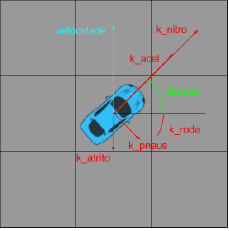
\includegraphics [scale = 1.2]{Forcas.PNG}
    \caption{Forças aplicadas no Carro}
\end{figure}

O histórico (listas de todas as posições em que o \emph{Carro} passou) e a lista com os tempos de cada jogador deve ser devidamente atualizada. 

O cerne desta Tarefa é a definicão da função \textbf{atualiza}. Quando recebe um \emph{Tempo}, um \emph{Jogo}, um \emph{Int} e uma \emph{Acao}, a função devolve o \emph{Jogo} correspondente.

\begin{verbatim}
    atualiza :: Tempo -> Jogo -> Int -> Acao -> Jogo

\end{verbatim}

\newpage
 \subsection{Tarefa 5}
Na tarefa 5, a biblioteca \textit{Gloss} adiciona a cada grupo, uma panóplia de funções que possibilitam a edição gráfica do jogo. O executável deve ser apelativo e cada grupo tem a liberdade de implementar funcionalidades originais na sua animação. Esperam-se jogos autênticos. 

Nesta tarefa, a função \textbf{movimenta} e \textbf{atualiza} serão fundamentais para o bom funcionamento dos carros.

Pretende-se a definição da função \textbf{main} que devolve um \emph{IO ()}

\begin{verbatim}
   main :: IO ()
\end{verbatim}

\subsection{Tarefa 6}
Por fim, na Tarefa 6 é esperado que cada grupo implemente uma estratégia de  jogo para a movimentação dos bots.
    Para tal é necessário ter em conta que :
\begin{itemize}
    \item O jogo acaba ao fim de 60 segundos Os mapas devem ser válidos de acordo com a Tarefa 2.
    \item São permitidos atalhos , tendo em conta que estes não permitem a ultrapassagem de mais de 4 peças.
    \item Cada jogador tem 5 segundos de nitro.
    \item Quando o \emph{Carro} é destruido, posteriormente, deve ser colocado no centro da última peça percorrida.
\end{itemize}

Para que isso aconteça é nessecária a definição da função \textbf{bot}, que dado um \emph{Tempo}, um \emph{Jogo} e um \emph{Int}, devolve a \emph{Acao} resultante.

\begin{verbatim} 
    bot :: Tempo -> Jogo -> Int -> Acao

\end{verbatim}

Análise sobre o que é pedido na fase 2 do projecto e qual é o problema em concreto.

\ldots


%% Descrição da Solução Desenvolvida
\chapter{A Nossa Solução}
\label{sec:solucao}

\section {Tarefa 1}
 A chave para a realização de um \emph{Mapa} concordante com o \emph{Caminho} fornecido foi a criação de um algoritmo capaz de colocar peças na posição adequada do \emph{Tabuleiro}.
 
 Na maior parte dos casos, a \emph{Peca} que se repete mais vezes no \emph{Tabuleiro} é a \emph{Peca Lava 0}, pelo que foi intenção do grupo, criar uma função que a colocasse em todas as posições do \emph{Tabuleiro}.
 Para tal, necessitou-se de considerar as dimensão do \emph{Tabuleiro} correspondente ao \emph{Caminho} dado.
 
 Dessa forma, a primeira função a ser criada foi a função \textbf{buildLava}.
 
 \begin{verbatim}
     buildLava :: Caminho -> Tabuleiro
     buildLava c = let x = fst (dimensao c)
                  y = snd (dimensao c)  
              in  replicate y (replicate x (Peca Lava 0))

 \end{verbatim}

A inserção de \emph{CurvaDir} e \emph{CurvaEsq} no Caminho, faz com que se altere a \emph{Orientação} que é tida em conta na construção das peças.

Devido a isso, houve a necessidade de elaborar uma função que colocasse as peças no local adequado, intitulada de \textbf{passosToPosition}. Devolve uma lista de \textbf{Peca} a partir de um Caminho. Tem em conta que a \emph{Orientação} inicial Este.

\begin{verbatim}
    passosToPosition:: Caminho -> [Posicao]
    passosToPosition [] = []
    passosToPosition c = positionEste (partida c) c

\end{verbatim}

Esta função está dependente de  outras 4 funções (\textbf{positionEste, positionOeste, positionNorte, positionSul}). Cada uma delas devolve a posição das peças segundo determinada \emph{Orientacao}. Recursivamente, devolvem as posições pretendidas.

Sob a influência do \emph{Caminho} está também a criação das peças que formam o Mapa. A \emph{Orientacao} volta a ser de novo fundamental, uma vez que o mesmo \emph{Passo} pode levar à execução de peças diferentes.

Para que a junção das peças seja a esperada ,comparativamente ao respectivo \emph{Caminho}, é necessário seguir um raciocínio similar ao da colocação das peças na \emph{Posicao} certa. Altera-se apenas os nomes das funções(\textbf{pecasEste}, \textbf{pecasOeste}, \textbf{pecasNorte}, \textbf{pecasSul}) que devolvem \textbf{Pecas}. A relação entre todas estas 4 funções irá ocorrer na função \textbf{passosToPecas}, que também considera a \emph{Orientacao} inicial Este.

\begin{verbatim}
    passosToPecas :: Caminho -> [Peca]
    passosToPecas [] = []
    passosToPecas c = pecasEste 0 c
 
\end{verbatim}

Para relacionar todas as funções descritas anteriormente, necessitou-se de ter uma função que fazia a substituição local de peças no \emph{Tabuleiro} de \emph{Lava}, apelidada de \emph{editTabuleiro}. Para executar o primeiro passo recursivo, a função \textbf{insertPeca} faz a alteração da \emph{Peca} numa \emph{Posicao} especifica do \emph{Tabuleiro}.

\begin{verbatim}
    editTabuleiro :: Tabuleiro -> [Peca] -> [Posicao] -> Tabuleiro
    editTabuleiro tab [] [] = tab
    editTabuleiro tab p ((x,y):t) = editTabuleiro 
    (insertPeca tab (head p) (x,y)) (tail p) t
\end{verbatim}

Por fim, na função \textbf{makeTabuleiro} ocorre a construção do \emph{Tabuleiro}. Com isto chegou-se à função objetivo (\textbf{controi}), que dá um \emph{Mapa} em função de um \emph{Caminho}.

\begin{verbatim}
    makeTabuleiro :: Caminho -> Tabuleiro
    makeTabuleiro c = editTabuleiro (buildLava c)
    (passosToPecas c)(passosToPosition c)
\end{verbatim}    

\begin{verbatim}
    constroi :: Caminho -> Mapa
    constroi c = Mapa (partida c, Este) (makeTabuleiro c) 
\end{verbatim}
  
\begin{table}[!h]
\begin{center}
\begin{tabular}{|l|c|r|}
    \hline
  \emph{Fases} & \emph{Descrição} & \emph{Função}\\
    \hline
  1º & Construção de um Tabuleiro de Lava & \textbf{buildLava} \\
  \hline
  2º & Posição das Peças & \textbf{passosToPosition} \\
    \hline
    3º & Escolhas das Peças & \textbf{passostoPecas} \\
    \hline
    4º & Alteração Local das Peças & \textbf{editTabuleiro} \\
    \hline
    5º & Construção do \emph{Tabuleiro} & \textbf{makeTabuleiro} \\
    \hline
    6º & Construção do \emph{Mapa} & \textbf{constroi} \\
    \hline
    
\end{tabular}
\end{center}

\caption{Fases da Resolução.}
\label{tbl:tabela}
\end{table}

Apresentar a solução para os problemas descritos em \ref{sec:analisefase1} e \ref{sec:analisefasee}.

\newpage

\section{Documentação}

O que tem um papel preponderante para o mais fácil entendimento do código redigido pelo grupo é a documentação, gerada automaticamente em Haddock.

O grupo teve em conta diversos fatores para que fosse visualmente apelativa e de fácil compreensão, tais como o facto de gerar um menu no canto superior direito da página, com uma divisão estruturada das funções consoante a fase do método de execução.

Mais a mais todas as funções apresentam pelo menos um exemplo explicativo, acompanhado de uma definição clara da sua funcionalidade. 





\begin{figure}[h!]
    \centering
    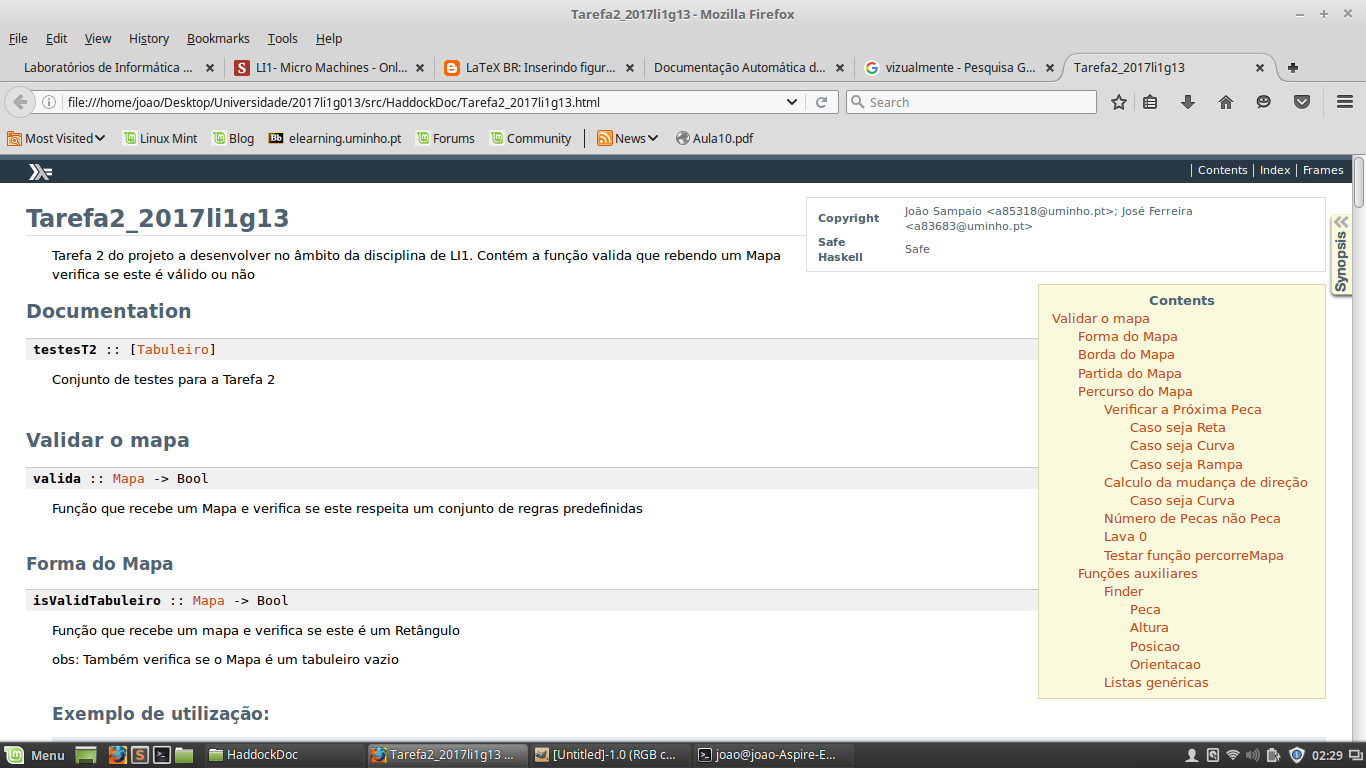
\includegraphics[scale = 0.2]{haddock.png}
    \caption{Documentação Haddock}
    \label{fig:my_label}
\end{figure}


% Como foi validada a implementação da solução
\chapter{Validação da Solução}

Aos alunos foi também disponibilizado um \emph{Sistema de Feedback}, ou seja, um repositório de controlo de versões (intitulado SVN), que permite que cada grupo coloque testes para verificar se o código que redigiram fornece os resultados esperados. Para além disso, recebem concelhos que visam a melhoria erros redundantes no código.

Na 1ºfase do projeto, a validação da solução tomada, baseou-se essencialmente nos resultados obtidos após a colocação de testes no SVN.

Descrever que abordagem tomaram para validar a solução apresentada na Secção \ref{sec:solucao}.

Em particular pode-se fazer uma descrição dos casos de teste
realizados para validar o desenvolvimento local.


\chapter{Conclusão}

\ldots

\bibliographystyle{plain}
\bibliography{bibliografia.bib}
\end{document}

